\section{Geodesics}
\label{sec:geodesics}

The main source of inspiration for this first chapter is the book by B. O'Neill \cite{o1983semi}. We shall refer mainly to chapters \(10\) and \(14\); when needed, more specific references will be made.

Let's start off with some basic concepts derived from differential geometry. We will generally address the spacetime manifold as \(M\), \(g\) its Lorentzian metric and \(\nabla\) the Levi-Civita covariant derivative.
We will generally assume that a \emph{spacetime} is a smooth, time-oriented Lorentzian manifold; we will use the terms manifold and spacetime interchangeably, unless otherwise stated.
The first fundamental definition we need is:
\begin{definition}
	Let \((M, g)\) be a spacetime and \(I \subseteq \R\) an interval; a smooth curve \(\gamma : I \rightarrow M\) is a \emph{geodesic} if its tangent field is parallel transported along \(\gamma\).
\end{definition}    

%\EAK{Below you are talking about timelike geodesics, clarify it and mention that the parametrization is proper time}

Restricting to the case of timelike geodesics parameterized by proper time, we may call \(U\indices{^{\mu}} \coloneqq \dot{\gamma}^{\mu}\) the tangent field, and the previous definition is equivalent to the equation:

\begin{equation}
\label{eq:tang-trans-fields}
\nabla_U U^{\mu} \coloneqq \frac{D\tensor{U}{^\mu} }{dt} \equiv 0.
\end{equation}



A \emph{curve} is a \(1\)-parameter map; similarly we can define a \emph{family of curves} as a \(2\)-parameter map \(\zeta: I \times J \rightarrow M\), where \(I, J \subseteq \R\) are intervals. This gives us \(2\) tangent fields, which we call respectively \emph{longitudinal} and \emph{transverse}:
\[
U^{\mu} \coloneqq \frac{\partial}{\partial t} \zeta^{\mu}(t,s); \quad \quad \quad 
V^{\mu} \coloneqq \frac{\partial}{\partial s} \zeta^{\mu}(t,s). 
\]

\begin{definition}
	Given a curve \(\gamma\), a \emph{(smooth) variation of \(\gamma\)} is any (smooth) \(2\)-parameter map \(\zeta(s,t)\) such that 
	\[
	\left. \zeta(s, t) \right\vert_{s = 0} = \gamma(t).
	\]
\end{definition}
An example is provided in figure \ref{fig:family-curves}.
\begin{figure}
	\caption[]{a smooth variation of a curve \(\gamma\) is a smooth family of curves \(\zeta\), such that \(\zeta\vert_{s = 0} \equiv \gamma\).}
	\label{fig:family-curves}
	\centering
	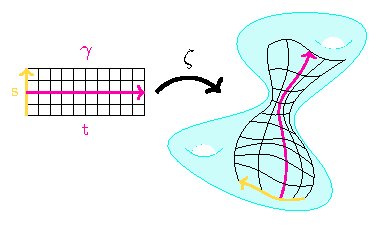
\includegraphics[scale=2.2]{Immagini/family-geodesics/family-geodesics.pdf}
\end{figure}

\begin{remark}
	Commutation of partial derivatives immediately gives 
	\[
	[U, V] = 0 \implies \nabla_U V^{\mu} = \nabla_V U^{\mu};
	\]
	secondly, by definition of the Riemann tensor,
	\[
	[\nabla_U, \nabla_V]W^{\mu} = R\indices{^{\mu}_{\nu\alpha\beta}}W^{\nu}U^{\alpha}V^{\beta}.
	\]
\end{remark}

By this remark we can compute the second derivative of the transverse field:
\[
\frac{D^2\tensor{V}{^\mu} }{dt^2} = \nabla_U\nabla_V U^{\mu} = \nabla_V\nabla_U U^{\mu} + R\indices{^{\mu}_{\nu\alpha\beta}}U^{\nu}U^{\alpha}V^{\beta}
\]

which leads us to the second fundamental object we need to define. 
\begin{definition}
	Given a family of \emph{geodesics} \(\gamma_s(t) \coloneqq \zeta(s,t)\), the transversal field \(V^{\mu} \coloneqq \frac{\partial}{\partial s} \zeta^{\mu}(t,s)\) is said to be a \emph{Jacobi field}.
\end{definition}

This vector field has a very important characterization, which here we'll only state:
\begin{lemma}
\(V^{\mu}\) is a \emph{Jacobi field} if and only if it satisfies the equation
	\begin{equation}
	\label{eq:Jacobi}
		\frac{D^2\tensor{V}{^\mu} }{dt^2} = \nabla_U\nabla_V U^{\mu} =  R\indices{^{\mu}_{\nu\alpha\beta}}U^{\nu}U^{\alpha}V^{\beta}.
	\end{equation}
\end{lemma}

Jacobi fields also have some nice properties we will find helpful in the prosecution of our work.
\begin{lemma}
	\label{lemma:Jacobi-fields-properties}
	Let \(V\) be a Jacobi field on \(\gamma\); then
	\[
	V \perp \gamma \iff \exists a\neq b \quad\vert\quad V\perp \gamma(a),\gamma(b) \iff \exists a \quad\vert\quad V, V' \perp \gamma(a).
	\]
\end{lemma}
\begin{proof}
	The proof is nearly straightforward from the characterization of Jacobi field and the symmetries of the Riemann tensor:
	\[
	\frac{d^2}{dt^2} (U^{\mu}V_{\mu}) = R_{\mu\nu\alpha\beta}U^{\mu}U^{\nu}U^{\alpha}V^{\beta} = 0
	\]
	hence \(U^{\mu}V_{\mu} = At + B\), from which the result is immediate.
\end{proof}


\section{Submanifolds}
\label{sec:submanifolds}

\begin{definition}
	Let \(M\) be a submanifold of the semi-Riemannian manifold \(\bar{M}\), and \(j:M\rightarrow\bar{M}\) the inclusion map. Then \(M\) is a \emph{semi-Riemannian submanifold} if the pullback of the metric tensor \(j^*(g)\) is a metric tensor on \(M\).
\end{definition}

This definition makes it clear that observers on the submanifold \(M\) agree on the notion of distance as if they were outside the submanifold. Nevertheless, observers within \(M\) see the world differently than observers from the outside: they in fact will inherit \(2\) different connections from their respective notion of metric. 

The comparison between these \(2\) different Levi-Civita connections gives surge to the \emph{second fundamental form}, which provides an infinitesimal description of the shape of \(M\) within \(\bar{M}\).

In order to introduce this important object notice first of all that:
\[
\forall p \in M \quad T_p\bar{M} = \underbrace{T_pM}_{\text{vectors tangent to }M}+ \underbrace{T_p(M)^{\perp}}_{\text{vectors orthogonal to } M}
\]

\noindent and we will generally call \(\Pi_p^{\parallel}\coloneqq d_pj\) and \(\Pi_p^{\perp}\coloneqq \mathbb{1} - d_pj\) the projective maps on these \(2\) subspaces.
Adopting a similar notation, we can decompose the set of all smooth fields in \(T\bar{M}\) restricted to \(M\) as:
\[
\bar{\mathfrak{X}}(M) = \mathfrak{X}(M) + \mathfrak{X}(M)^{\perp}.
\]

Now, the connection \(\bar{D}\) on \(\bar{M}\) will naturally give raise to a connection on \(M\)
\begin{align*}
\bar{D} : \mathfrak{X}(M) \times \bar{\mathfrak{X}}(M) & \rightarrow \bar{\mathfrak{X}}(M) \\
	 V \times X &\mapsto \bar{D}_V X
\end{align*}

by taking any smooth extension of the fields \(V\) and \(X\) to \(\mathfrak{X}(\bar{M})\), and then restricting again on \(M\). It can be proved that \(\bar{D}_V X\) is a well-defined smooth vector field on \(M\). In particular
\begin{lemma} 
	if \(V, W \in \mathfrak{X}(M)\) and \(D\) is the Levi-Civita connection on \(M\), it holds that
	\[
	D_V W = \Pi^{\parallel}\left(\bar{D}_V W\right).
	\]
\end{lemma}

It's evident then that the Levi-Civita connection on \(M\) is missing something with respect to the induced connection from \(\bar{M}\). This is precisely the object we have been looking for:

%\EAK{Math symbol for second fundamental form: $\mathrm{I\!I}$}
\begin{definition}
	given \(M \subset \bar{M}\) a semi-Riemannian submanifold, the \emph{shape tensor} (or \emph{second fundamental form}) is defined as:
	\begin{align*}
		\mathrm{I\!I} : \mathfrak{X}(M) \times \mathfrak{X}(M) &\longrightarrow \mathfrak{X}(M)^{\perp}\\
							V \times W &\mapsto \Pi^{\perp}\left(\bar{D}_V W\right)
	\end{align*}
	\noindent and in particular is bilinear and symmetric.
\end{definition}

In order to gain a better understanding of what this object encodes, let's think for a moment about the following example. Given a field \(Y \in \mathfrak{X}(M)\) tangent to a curve \(\alpha\) of \(M\), parameterized by \(s\), we indicate:
\[
\dot{Y} \coloneqq \frac{\bar{D}Y}{ds} \quad \quad Y' \coloneqq \frac{DY}{ds}
\]
It is then easy to prove that:
\[
\ddot{\alpha} = \alpha'' + \mathrm{I\!I}(\alpha', \alpha')
\]

and hence, we can think of \(\mathrm{I\!I}\) as the additional external ``force'' needed to prevent a point from leaving \(M \subset \bar{M}\), a sort of constraining force.
This can be visualized witn the example in figure \ref{fig:shape-tensor}: any particle moving on the yellow curve would leave \(M\) unless an external force - such as the yellow vector - is applied.
Finally, an equivalent interpretation of \(\mathrm{I\!I}\) is by how much a vector paralleled transported in \(M\) according to \(D\) is actually changing from the point of view of \(\bar{D}\).

\begin{figure}
	\caption[]{Vector fields \(V\) and \(W\) belong to \(\mathfrak{X}(M)\) and generate respectively the cyclamen and the yellow curve. The \(2\) vectors represent the shape tensor evaluated in these \(2\) vectors, and clearly bear the interpretation of constraing force introduced above.}
	\label{fig:shape-tensor}
	\centering
	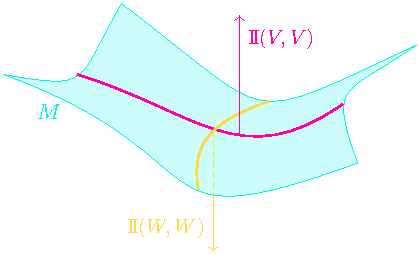
\includegraphics[scale=1.7]{Immagini/shape-tensor/shape-tensor.pdf}
\end{figure}

We now prove an identity which will be useful to remember in the future. First of all we need to define the analogous of Jacobi fields for variations of curves where one of the endpoints is a submanifold: the \(M\)-Jacobi fields.
\begin{definition}
	Given a submanifold \(M\) in \(\bar{M}\), a \(M\)-Jacobi field is the variation vector field of a geodesic \(\gamma \perp M\) through normal geodesics.
\end{definition}
\begin{lemma}
	\label{lemma:shape-identity}
	Let \(M\) be a submanifold of \(\bar{M}\), \(\gamma\) a curve leaving \(M\) orthogonally at \(p\), with tangent vector field \(U^{\mu}\), and \(e_1, \ldots, e_m\) a basis for the space of perpendicular \(M-\)Jacobi fields on \(\gamma\).
	Then 
	\begin{equation}
		(\Pi^{\parallel}\nabla_Ue_i)_{\mu}e_j^{\mu} = - \mathrm{I\!I}(e_i, e_j)^{\mu}U_{\mu}
	\end{equation}
\end{lemma}

	\begin{proof}
		As \(\gamma\) and its variations are orthogonal to \(M\) \(e_j^{\mu}U_{\mu} \equiv 0\), hence:
		\[
		0 = \nabla_{e_i}\left(e_j^{\mu}U_{\mu}\right) = \left(\nabla_{e_i}U_{\mu}\right)e_j^{\mu} + U_{\mu}\left(\nabla_{e_i}e_j^{\mu}\right)
		\]
		Again, \(U_{\mu}\) is orthogonal to \(M\), then \(U_{\mu}  \left(\nabla_{e_i}e_j^{\mu}\right)= U_{\mu}\left(\Pi^{\perp}\nabla_{e_i}e_j^{\mu}\right)\), while \(e_i\) is a Jacobi field so \(\nabla_{e_i}U^{\mu} = \nabla_Ue_i^{\mu}\). Plugging this back into the previous equation we get exactly
		\[
		(\Pi^{\parallel}\nabla_Ue_i)_{\mu}e_j^{\mu} = (\nabla_Ue_i)_{\mu}e_j^{\mu} = (\nabla_{e_i}U)_{\mu} e_j^{\mu} = - U_{\mu}\left(\Pi^{\perp}\nabla_{e_i}e_j^{\mu}\right) = - \mathrm{I\!I}(e_i, e_j)^{\mu}U_{\mu}.
		\]
	\end{proof}


The second fundamental form induces a vector field on \(M\) called \emph{mean curvature}.


\begin{definition}
		Let \(M \subset \bar{M}\) be an \(n\)-semi-Riemannian submanifold, with \emph{shape tensor} \(\mathrm{I\!I}\), and \(\{\textbf{e}_i\}_{i \in \{1, \ldots, n\}}\) any frame on \(M\) at \(p\). Then we call \emph{mean curvature vector field} the field \(\mathrm{H} \in \mathfrak{X}(M)^{\perp} \) defined by:
		\[
		\mathrm{H}^{\mu}(p) = \frac{1}{n} \sum_{i=1}^{n} \epsilon_i \mathrm{I\!I}^{\mu}(\textbf{e}_i, \textbf{e}_i).
		\]
		where 
		\[
		\epsilon_i = 
		\begin{cases}
		+1 \quad \text{if } \textbf{e}_i \text{ is \emph{timelike}} \\
		-1 \quad \text{if } \textbf{e}_i \text{ is \emph{spacelike}}
		\end{cases}
		\]
\end{definition}

This definition will be particularly important for the proof of the Null Singularity theorem and the Black Hole Area theorem, as they are instrumental to define the concept of a \emph{trapped surface}, the initial condition needed to eventually develop a singularity (in the classical limit). 

Finally, let us prove a quick lemma that will be useful here and there throughout the all analysis of the thesis.
\begin{lemma}
	\label{lemma:metric-decomposition}
	Let \(P\) be a spacelike hypersurface of codimension \(2\) and \(\gamma_s\) a congruence of null geodesics leaving normally from \(P\); call \(U^{\mu}\) the (null) tangent vector field and \(\{e_i^{\mu}\}_{i = 1, \ldots, n - 1}\) an orthonormal basis of the tangent space to \(P\). Finally, parallel transport \(\{e_i^{\mu}\}_{i = 1, \ldots, n - 2}\) along \(\gamma\) in order to gain \(n - 2\) vector fields \(\{E_i^{\mu}\}_{i = 1, \ldots, n - 2}\). Then there exists a null vector field \(W^{\mu}\) such that the metric can be decomposed as
	\begin{equation}
		g^{\mu\alpha} = U^{\mu}W^{\alpha} + U^{\alpha}W^{\mu} - \sum_{i=1}^{n - 2}E_i^{\mu}E_i^{\alpha}.
	\end{equation}
\end{lemma}

\begin{proof}
	This is only a linear algebra exercise, which basically reduces to decompose the metric tensor on \(T_{\gamma_0}M = T_{\gamma(0)}P \oplus T_{\gamma(0)}P^{\perp}\). By definition \(\{E_i^{\mu}\}_{i = 1, \ldots, n - 2}\) is an orthonormal basis of \(T_{\gamma(0)}P\), so we are left with the decomposition on \(T_{\gamma(0)}P^{\perp}\), whose dimension is \(2\) by hypothesis.
	We already know that a non degenerate vector in \(T_{\gamma(0)}P^{\perp}\) is \(U^{\mu}\) and as the signature is \((+, -)\), then there must be another null vector \(W^{\mu}\) such that \(W^{\mu}U_{\mu} = 1\) (we can think about \(\R^{1,1}\) as it's always possible to reduce to that for the tangent space of a single point). Now we have found a basis of \(T_{\gamma_0}M\), and it's easy to show that for any \(2\) vectors \(a\) and \(b\) we can decompose them in terms of this new basis, compute their inner product using both formulations of \(g\), and check they are equal.
\end{proof}

\section{Trapped surfaces}

\begin{definition}
	\label{def:trapped-surface}
	We say that a spacelike submanifold \(P\) is \emph{future-converging} or \emph{future-trapped} provided its mean curvature vector field \(\mathrm{H}\) is past-pointing timelike.
\end{definition}


It is only a matter of simple linear algebra in each normal space \(T_p(P)^{\perp}\) to show that
\begin{lemma} \label{lemma:charact-trapped}
	assuming \(P\) is a \emph{spacelike} submanifold, the following statements are equivalent:
	\begin{enumerate}
		\item  \(k(v) =\mathrm{H}^{\mu} v_{\nu} < 0 \) for all future pointing \emph{null} vectors \(v\) normal to P.
		\item  \(k(w) =\mathrm{H}^{\mu} w_{\nu} < 0 \) for all future pointing \emph{causal} vectors \(w\) normal to P.
		\item \(\mathrm{H}\) is past-pointing timelike.
	\end{enumerate}
\end{lemma}

\begin{proof}
	We will prove a chain of implications to gain the equivalence.
	
	\(\mathbf{2) \implies 1)]}\) this is trivial because any null vector is a causal vector.
	
	\(\mathbf{1) \implies 3)]}\) Let's write \(\mathrm{H}^{\mu} = (\mathrm{H}^0, \vec{\mathrm{H}})\). It is possible to choose a spacelike \(3-\)vector \(\vec{v}\) such that \(\vert\vec{v}\cdot\vec{\mathrm{H}}\vert = - \vert\vec{v}\vert\cdot\vert\vec{\mathrm{H}}\vert\) and  then complete it to the future-pointing null vector \(v^{\mu} = (v^0, \vec{v})\) (where \(v^0 = \vert \vec{v}\vert > 0\)).
	Now:
	\[
	\mathrm{H}^{\mu}v_{\mu} = \mathrm{H}^0v^0 - \vec{\mathrm{H}}\cdot\vec{v} < 0 \quad \implies 
	\quad v^0 \mathrm{H}^0 < - \vert\vec{v}\vert\cdot\vert\vec{\mathrm{H}}\vert < 0
	\]
	which, for the positivity of \(v^0\), implies that \(H^{\mu}\) is timelike and past-pointing.
	
	\(\mathbf{3) \implies 2)]}\) first of all observe that any causal vector can be written as the sum of \(2\) future-pointing vectors such that \(w^{\mu}= v^{\mu} + t^{\mu}\) where \(v\) is null, and \(t^{\mu} = (t^0, \vec{0})\) (with \(t^0 \ge 0\)). At this point:
	\[
	w_{\mu}\mathrm{H}^{\mu} = v_{\mu}\mathrm{H}^{\mu} + \underbrace{t^0 \mathrm{H}^0}_{\le0}
	\]
	Moreover, by Cauchy-Schwartz we have:
	\[
	v_{\mu}\mathrm{H}^{\mu} = v^0 \mathrm{H}^0 - \vec{\mathrm{H}}\cdot\vec{v} \le v^0\mathrm{H}^0 +\vert \vec{\mathrm{H}}\vert\cdot\underbrace{\vert\vec{v}\vert}_{v^0} = v^0\underbrace{(\mathrm{H}^0 + \vert \vec{\mathrm{H}}\vert)}_{<0} < 0.
	\]
\end{proof}

However, the one stated above \ref{def:trapped-surface} is not the definition that has been in use from the beginning of the analysis of these objects. The most widely used definition is by far the one that passes through the definition of expansion: we will now state this definition for codimension \(2\) spacelike submanifolds, and making use of the \emph{null} expansion, but the same idea can be generalized to a much larger class of submanifolds. Consider the spacelike codimension \(2\) submanifold \(P\subset M\), and the congruence of \emph{null} geodesics leaving normally from \(P\); call \(U^{\mu}\) the tangent field.

Of course there are \(2\) such congruences: we will call \emph{positive} congruence one of them, and \emph{negative} the other one, whose tangent field - except for riparametrization - will be \(W^{\mu}\). By lemma \ref{lemma:metric-decomposition} we can decompose the metric as 
\[
g^{\mu\alpha} = U^{\mu}W^{\alpha} + U^{\alpha}W^{\mu} - \sum_{i=1}^{n - 2}E_i^{\mu}E_i^{\alpha}.
\]
Moreover,
\begin{definition}
	 Consider the tensor field given by the gradient of the tangent field:
	\[
	B_{\mu\nu} = \nabla_{\nu}U_{\mu}.
	\]
	The trace of \(B_{\mu\nu}\) is going to be called \emph{positive null expansion}:
	\[
	\theta^{+} = \texttt{tr}\left[B\right] = g^{\mu\nu}B_{\mu\nu}.
	\]
	Similarly, if we chose the negative congruence we would have had
	\[
	\tilde{B}_{\mu\nu} = \nabla_{\nu}W_{\mu}.
	\]
	and its trace is defined as the \emph{negative null expansion}
	\[
	\theta^{-} = \texttt{tr}\left[\tilde{B}\right] = g^{\mu\nu}\tilde{B}_{\mu\nu}.
	\]
\end{definition}

It's clear that for any point of the submanifold we are able to compute the positive and the negative expansion; this finally leads to the definition of trapped surface
\begin{definition}
	A codimension \(2\) spacelike hypersurface is called \emph{trapped} if both its positive and negative expansions are negative
	\[
	\theta^+ , \theta^- < 0.
	\]
\end{definition}

We finally want to prove that the \(2\) definitions are indeed equivalent.
\begin{lemma}
	\label{lemma:equiv-trapped}
	The \(2\) definitions of trapped surface are equivalent.
\end{lemma}
\begin{proof}
	Let us use the same notation introduced above, for which \(P\) is the hypersurface under consideration, \(\{E_i^{\mu}\}_{i = 1, \ldots, n - 2}\) is an orthonormal basis of its tangent space, \(U^{\mu}\) and \(W^{\mu}\) \(2\) orthogonal null vectors such that \(U^{\mu}W_{\mu} = 1\) tangent to the respective orthogonal null congruences. As \(U^{\mu}\) is null and parallel transported we have
	\begin{align*}
		\theta^+ &= g^{\mu\nu}B_{\mu\nu} = \left(g^{\mu\nu} - U^{\mu}W^{\nu} - U^{\nu}W^{\mu}\right)B_{\mu\nu} =\\
		&= - \sum_{i=1}^{n - 2}E_i^{\mu}E_i^{\nu}B_{\mu\nu} = - \sum_{i=1}^{n - 2}E_i^{\mu}E_i^{\nu}\nabla_{\nu}U_{\mu} = \\
		& = -  \sum_{i=1}^{n - 2}E_i^{\nu}\nabla_{\nu}\underbrace{\left(E_i^{\mu}U_{\mu}\right)}_{0} +  \sum_{i=1}^{n - 2}U_{\mu}E_i^{\nu}\nabla_{\nu}E_i^{\mu} = \sum_{i=1}^{n - 2}U_{\mu}\nabla_{E_i}E_i^{\mu} = \\
		& = (n - 2) U_{\mu} \cdot \frac{1}{n - 2}\sum_{i=1}^{n - 2}\mathrm{I\!I}^{\mu} \left(E_i, E_i\right) = (n - 2) U_{\mu}\mathrm{H}^{\mu}.
	\end{align*}
	Similarly
	\[
	\theta^- = (n - 2) W_{\mu}\mathrm{H}^{\mu}.
	\]
	As \(P\) has codimension \(2\), \(U^{\mu}\) and \(W^{\mu}\) are the only independent null vectors orthogonal to \(P\), and then, by means of lemma \ref{lemma:charact-trapped}, we know that 
	\[
	\theta^+ , \theta^- < 0 \iff \mathrm{H}^{\mu} \text{ is past-pointing timelike,}
	\]
	establishing the equivalence between the \(2\) definitions.
\end{proof}

\begin{remark}
	It's worth pointing out that, as Wald states in section \(9.2\) of \cite{wald2010general} about the expansion of a null congruence of geodesics, there is no natural way to directly compute \(\theta\), as we have done above. The point is that we didn't have only the congruence, but also a submanifold \(P\) to which the congruence is orthogonal, and that indeed infers a natural basis with which is possible to compute \(\theta\). Given only the congruence instead, there are infinitely many possible spacelike submanifolds orthogonal to it, as one can see by studying the system in \(R^{2,1}\).
	%todo: fai disegno sulle note del 17/04
	\begin{figure}[!h]
		\centering
		\includegraphics[scale=1.7]{example-image-duck}
	\end{figure}
\end{remark}


Even if we already have \(2\) good definitions of \emph{trapped} surface, they are both rather mathematical, while we would like to develop a better intuition of the features of these objects. The most outstanding property is described by the following lemma; we report the statement given in \cite{senovilla2022critical}. A proof for hypersurfaces of codimension \(1\) can be found in \cite{kriele1999spacetime} as Lemma \(4.4.8\), and can be generalized to submanifolds of any dimension, but we don't report the proof here.
\VS{Should I write the proof of this fact here?}
\begin{lemma}
	\label{lemma:variation-area}
	Let \(P\) be any spacelike submanifold of any dimension, and denote as \(\mathcal{A}_P\) its area. Then choose an arbitrary vector field \(\xi^{\mu}\): this will induce a flow \(F_t\), and \(P\) can be deformed along this flow. The initial variation of the area due to this deformation is
	\[
	\delta_{\xi}\mathcal{A}_P = \int_{P} \texttt{div}_P (\Pi^{\parallel}\xi) + \mathrm{H}^{\mu}\xi_{\mu}.
	\]
\end{lemma}
 Clearly, if \(P\) is without boundary the first term integrates out for Stokes theorem (\(\texttt{div}_P\) is the divergence of \(P\)), and we are left with
 \begin{equation}
 	\label{eq:variation-area}
 	\delta_{\xi}\mathcal{A}_P = \int_{P} \mathrm{H}^{\mu}\xi_{\mu}.
 \end{equation}
	This equation is telling us that \(P\) is trapped if and only if its area is doomed to decrease, no matter how they evolve (as long as they keep causality). In this sense they are trapped, or rather, \emph{trapping}, because everything they contain will be surrounded by a submanifold of less and less area... Until some catastrophe might occur!

\section{Causal structure}

The notion of \emph{causality} has to do with the fact that in a Lorentzian manifold, starting from a  point \(p\) it is not true that an observer or a light ray can travel to any other point \(q\), as they are only allowed to move along (future pointing) causal geodesics (i.e. whose tangent field is never spacelike).

First of all it is important to define what we mean by ``future'' and ''past''. For any given \(p\in M\) the tangent space \(V_p\) is isomporhic to Minkowski spacetime, and hence we are able to define the light cone contained in \(V_p\) through its origin. We will call that the \emph{light cone of} \(p\): note that this is a subset of \(V_p\) and not of \(M\) as for the \emph{null cone}.
Now, for each \(p\) we can choose one half of the light cone to be the ``future'' and the other half to be the ``past''; we would also like to make a choice which is continuous and self-consistent, but this is not always possible!

\begin{figure}
	\centering
	\includegraphics[scale=1.7]{example-image-duck}
	%todo: aggiungi figura di spazio non time orientable -- Wald pag 189 fig. 8.1
\end{figure}
We will call \((M, g_{\mu\nu})\) \emph{time-orientable} if such a  choice can be pursued; in the following we will always assume that the manifold under consideration is time-orientable, otherwise we would have to deal with the highly unphysical case of not being able to distingiush between the notions of moving ``forward in time'' or ``backward in time''.

We will denote causality relations with the following notation, following \cite{o1983semi}.
\begin{enumerate}
	\item  \(p \pprec q\) means there is a future-pointing \emph{timelike} curve in \(M\) connecting \(p\) to \(q\).
	\item \(p \prec q\) means there is a future-pointing \emph{causal} curve from \(p\) to \(q\); \(p \preceq q\) means either \(p \prec q\) or \(p = q\).
\end{enumerate}

Evidently \(p\pprec q\) implies \(p\prec q\) but not vice versa. For a subset \(A \subseteq M\) we also define:
\begin{enumerate}
	\item the \emph{chronological future} of \(A\)
	\[
	I^+(A) =\{ q\in M :\quad\exists p \in A\text{ with } p\pprec q\}.
	\]
	These are events that can be reached for a massive particle starting at \(p\); for the stability of the timelike characterization under small perturbations of curves it's clear that \(I^+(p)\) is always an open set.
	\item the \emph{causal future} of \(A\)
	\[
	J^+(A) =\{ q\in M : \quad\exists p \in A\text{ with } p\preceq q\}.
	\]
	These are events that, in principle, can be influenced by any signal emitted in \(p\). In Minkowski spacetime \(J^+(p)\) is always closed, but conversely from before, this doesn't generalize to arbitary spacetimes (simple counterexamples are given by Minkowski without a point).
\end{enumerate}
By reversing time orientation we get the corresponding \emph{past} definitions and from any proof for \emph{future} versions it's possible to infer the analogous for past ones.

In Minkowski spacetime \(I^+(p)\) consists of exactly of the points that can be reached by future directed timelike \emph{geodesics} starting from \(p\), and the boundary \(\partial I^+(p)\) is generated by future directed \emph{null} geodesics (starting from \(p\)). In general neither of this statement is true, but they hold \emph{locally}: a formal statement and proof of this result is due to Hawking and Eliis and can be found in \cite{hawking1973large} as proposition \(4.5.1\).

What we are really interested in though is the following corollary, that follows immediately from the property above mentioned.
\begin{corollary}
	If \(q \in J^+(p) \setminus I^+(p)\), then any causal curve connecting \(p\) to \(q\) must be a null geodesic.
\end{corollary}

\begin{proof}
	If \( q \in J^+(p)\) and \(\gamma\) is a causal curve beginning at \(p\) and ending a \(q\), we can cover \(\gamma\) by convex normal neighborhood and then, since \(\gamma\) is compact, extract a finite subcover.
	
	If \(\gamma\) failed to be a null geodesic in any of these neighborhoods we could deform it to a \emph{timelike} curve in that neighborhood, and then extend this deformation to the other ones, to obtain a timelike curve from \(p\) to \(q\). Hence \(q\) would be in \(I^+(p)\) as well.
\end{proof}

With similar arguments we have that \(J^+(A) \subseteq \bar{I}^+(A)\), and since clearly \(I^+(A) \cup A \subseteq J^+(A)\) it's clear that \(\overline{J^+(A)} = \overline{I^+(A)}\) and \(\partial J^+(A) = \partial I^+(A)\).

\subsection{The boundary of the future}
Given a submanifold \(A\), \(\partial J^+(A)\) will be called the \emph{boundary of the future} of \(A\): this is again a \(3-\)sumbanifold and has some interesting properties. As we will often work with this object it makes sense to stop for a moment and highlight some of its features.

\begin{definition}
	A set \(S\in M\) is said to be \emph{achronal} if there do not exist \(p, q \in S\) such that \(q\in I^+(p)\), or in other words \(p\) and \(q\) must not be joinable via a timelike curve. 
\end{definition}

\begin{remark}
	There is no mutual implication between achronality and signature of the submanifold \(S\).
	It is pretty clear that achronality doesn't imply that \(S\) needs to be spacelike (the following will provide an example), but a spacelike submanifold doesn't need to be achronal either. The most famous example is given by the cilynder spacetime, whose vertical axes is the time direction.

	\begin{figure}
	\centering
	\begin{tikzpicture}
	\coordinate (a) at (0,0);
	\coordinate (b) at (1.4,0);
	\coordinate (c) at (0,2.2);
	\coordinate (d) at (1.4,2.2);
	\coordinate (e) at (1.4, 0.8);
	\coordinate (f) at (0, 1.6);
	\coordinate (g) at (0.7, 1.9);
	\coordinate (h) at (0.7, 0.20);
	\draw (a)--(c);
	\draw (b)--(d);
	\draw[dashed] (0,0) arc (180:0:0.7 and 0.3);
	\draw (0,0) arc (180:360:0.7 and 0.3);
	%\draw[dashed] (0.7, 0) ellipse (0.7 and 0.3);
	\draw (0.7, 2.2) ellipse (0.7 and 0.3);
	\draw[fuchsia] (a) to [out = 15, in = -115] (e);
	\draw[dashed, fuchsia] (e) to [out = 125, in = -20] (f);
	\draw[fuchsia] (f) to [out = 15, in = -145] (g);
	\draw[thick, turquoise] (h) -- (g);
	\foreach \i in {h,g} {\fill[turquoise] (\i) circle(.8pt);}
	\node[below] at (h) {\footnotesize\(p\)};
	\node[above] at (g) {\footnotesize\(q\)};
	\node[left] at (f) {\footnotesize\(S\)};
	
	\end{tikzpicture}
	\caption{\(t = \epsilon\phi\) is not achronal but can be spacelike.}
\end{figure}

\end{remark}

\begin{theorem}
	Let \((M, g_{\mu\nu})\) be a time orientable spacetime and let \(S\subset M\). Then \(\partial J^+(S)\) (if nonempty) is an achronal, three-dimensional embedded submanifold of \(M\).
\end{theorem}
\begin{proof}
	We'll prove only the achronality part because it's the one that is most intersting to 
	us, and we refer to the proof in O'Neill \cite{o1983semi} (which applies in general 
	to any future set). Clearly \(I^+(S) \subseteq I^+(I^+(S))\); 
	let \(p\in \partial J^+(S)\) and \(q \in I^+(p)\): then \(p \in I^-(q)\) and 
	whole open neighborhood \(O\)  of \(p\) will be contained in \(I^-(q)\), 
	because \(I^-(q)\) is open. 
	Since \(p\) is in \(\partial I^+(S)\) \(O \cap I^+(S) \neq \emptyset\), \(q\) 
	is to the future of some points in \(I^+(S)\) as well - \(q \in I^+(O \cap I^+(S)) \) -
	 hence \(I^+(p) \subseteq I^+(S)\). 
	 Similarly \(I^-(p) \subseteq M \setminus I^+(S)\).
	
	Now, if \(\partial I^+(S)\) failed to be achronal, we could have 
	\(q,r \in \partial I^+(S)\) such that \(r \in I^+(q)\); but this would imply 
	\(r \in I^+(S)\) and \(r \in \partial I^+(S)\) at the same time, which is a 
	contradiction as \(I^+(S)\) is open, which is 
	\(I^+(S) \cap \partial I^+(S) = \emptyset\).
\end{proof}

Curves on this submanifold are, in some weak sense, protected from ending: none of the points in \(\partial I^+(S)\) is able to prevent a curve from being extended further. To prove this statement precisely we need to introduce the concept of \emph{endpoint}.
	\begin{definition}
		A point \(p\in M\) is a \emph{future endpoint} of a curve \(\gamma\) if for every neighborhood \(O\) of \(p\) there exists a \(t_0\) such that \(\gamma(t) \in O \quad \forall t >t_0\). 
		
		A curve is said to be \emph{future inextendible} is it has no future endpoint.
	\end{definition}

	This concept of future inextendibility locally can pass to the limit, 
	so it is possible to prove the following important result:
\begin{theorem}
	\label{th:null-generator}
	Let \(C\) be a \emph{closed} subset of the spacetime manifold \(M\). 
	Then every point in \(p\in \partial I^+(C)\) with \(p \notin C\) lies on a null 
	geodesic \(\gamma\) which lies entirely in \(\partial I^+(C)\) and either is 
	past inextendible or has a past endpoint on \(C\). Such geodesics are called \emph{null generators} of \(\partial J^+(C)\).
\end{theorem}

The proof can be found in many books and doesn't add a particular insight, so we 
decided not to include it, but the curious reader might look at chapter \(8\) 
of \cite{wald2010general}. 
Notice that this theorem is \emph{not} saying that if we are lying on \(\partial I^+(C)\) 
there exists a light ray that travels from \(C\) to us: a good example is provided by
\(\R^{1,1}\) with a point removed, and is shown in fugure
\begin{figure}
	\centering
	\includegraphics[scale=1.7]{example-image-duck}
	%todo: tipo figura pag.191 Wald
	\caption{the curve on the left side of the cone is not able to reach \((0,0)\), but
	is past inextendible since its past endpoint would be \((-1, 1)\), which doesn't belong
	to the manifold though.}
\end{figure}
Indeed this property of ``completeness'' of \(\partial I^+(C)\) is in general non trivial to gain, and it requires some extra assumptions about the manifold. Such assumptions are exactly the causality conditions.

\subsection{Causality Conditions}
Even if all spacetimes have \emph{locally} the same causal structure as Special Relativity, globally things can change dramatically.

The first, minimal requirement that we want to ask for is that \(M\) does not contain any  closed timelike curve; this is called the \emph{chronology condition}, and its failure would lead to some distressing paradoxes (one of the most famous is that an observer might take a trip to the past, kill one of its own ancestors and so prevent his own birth).

\begin{lemma}
	If \(M\) is compact, it contains a closed timelike curve.
\end{lemma}
The previous lemma makes us restrict to the study only of non compact manifolds.
Slightly strentenighing the condition we have been talking about up to now we obtain the \emph{causality condition}, which asks \(M\) not to contain any closed \emph{causal} curve. This of course implies the chronology condition, but is not equivalent to it; however, even if a spacetime doesn not posses any closed causal curve it might still be ``on the verge'' of violating causality since there might be some causal curves that go arbitrarly close to interesct themselves.

Such spacetimes are not considered physically resonable either because a small perturbation of the metric might actually break causality, so we want to rule out this possibility as well. One way to do so is asking for \emph{strong causality}.
\begin{figure}
	\centering
	\includegraphics[scale=1.7]{example-image-duck}
	%todo: inserisci esempio fig. 8.8 pag.197 wald
\end{figure}
\begin{definition}
	\emph{Strong causality} holds at \(p\in M\) provided that given any neighborhood \(U\) of \(p\), there is a neighborhood \(V\subset U\) of \(p\) such that every causal curve segment with endpoints in \(V\) lies entirely in \(U\).

	A spacetime is \emph{strongly causal} if strong causality holds for any \(p\in M\).
\end{definition}

	It is clear that if strong causality is violated at \(p\), then near \(p\) there exist causal curves arbitrarly close to intersecting themselves; at the same time it can be easily proved that in a strongly causal spacetime, if a causal curve leaves a compact \(K\subset M\), it can never return to it, so no curve can ever return arbitrarly close to itself.

	Although strong causality implies causality, and suffices to rule out pathological cases as the ones mentioned before, it is still possible that modification of \(g_{\mu\nu}\) in arbitrarly small neighborhoods of \(1\) or more points produces closed causal curve. We need to refine further the conditon we ask for, to be sure we are never on the verge of producing causality violation. Such a condition is \emph{stable causality}:
	\begin{definition}
		A spacetime \((M, g_{\mu\nu})\) is \emph{stably causal} if there exists a timelike non-vanishing vector field \(X^{\mu}\) such that \((M, \tilde{g}_{\mu\nu})\) possess no closed timelike curves, where
		\[
			\tilde{g}_{\mu\nu}= g_{\mu\nu} - X^{\mu}X^{\nu}.
		\]
	\end{definition}
	The idea behind this definition is that, by defining \(\tilde{g}_{\mu\nu}\), we are ``opening up'' the light cone, so if we were ``on the verge'' of violating causality now we are definitely not able to avoid it. As a reference, this definiton is equivalent to the following condition:
	\begin{theorem}
		\label{th:stable-causality}
		A spacetime \((M, g_{\mu\nu})\) is \emph{stably causal} if and only if there exists a differentiable function \(f\) of \(M\) such that \(\nabla^{\mu}f\) is a past-directed timelike vector field.
	\end{theorem}
By theorem \ref{th:stable-causality} it is possible to see that stable causality implies strong causality, and this finally appears to be the notion of not being close to break causality.

We concluded the previous subsection by saying that we will need causality to be linked to some notion of ``completeness'' of set of curves. In order to approach that let's define the concept of \emph{time separation}.
\begin{definition}
	If \(p,q\in M\) the \emph{time separation} \(\tau (p,q)\) from \(p\) to \(q\) is
	\[
		\tau (p,q) = \sup{L(\gamma): \gamma\text{ is a future pointing causal curve segment from } p \text{ to } q}.
	\]
\end{definition}
We can think of \(\tau (p,q)\) as the proper time of the slowest trip in \(M\) from \(p\) to \(q\), and is sort of the dual of distance for Riemannian geometry.
Similarly, time separation between sets of points is obtained by taking the supremum of \(\tau\) over the all set. Now,
\begin{prop}
	\label{prop:global-existence}
	For \(p \prec q\), if the set \(J(p, q) = J^+(q) \cap J^-(q)\) is compact and strong causality holds on it, then there exists a causal geodesic from \(p\) to \(q\) of length \(\tau (p,q)\).
\end{prop}
When reduced to the timelike case, this theorem guarantees the existence of the actual path an inertial observer will follow from \(p\) to \(q\), and applying the analysis of chapter \ref{ch:focal-points} to the lenght functional would lead us to conclude that such curves must have no focal or conjugate point. For causal curves in general the link is not as direct, and more care needs to be payed, but we will try to shed some light on this correspondence in section \ref{sec:promptness}.

Moreover, this is exactly what we need to extend theorem \ref{th:null-generator}: now \(\forall p\in \partial I^+(C)\)  there exists a null generators through \(p\) that intersect \(C\) \emph{and} it doesn't contain any focal point (see lemma \(14.30\) of \cite{o1983semi}).
Indeed proposition \ref{prop:global-existence} motivates the following fundamental definition:
\begin{definition}
	\label{def:global-hyper}
	a subset \(V\) of \(M\) is globally hyperbolic if 
	\begin{enumerate}
		\item strong causality holds on \(V\);
  		\item for all \(p, q \in V\) such that \(p \prec q\) \(J(p,q)\) is compact and contained in \(V\).
	\end{enumerate}
\end{definition}

We already understand why \ref{def:global-hyper} is an important definition, but it is not equally evident why we should denote that as a causality condition: an equivalent formulation is going to clear this out.

\subsection{Domains of dependance}
Let \(S\) be a closed achronal set (this is a techincal requirement); then
\begin{definition}
	The \emph{future domain of dependance} of \(S\), denoted by \(D^+(S)\), is defined as
	the set of points \(p\in M\) such that every past inextendible causal curve through \(p\) intersects \(S\).
\end{definition}

The idea behind this definition is due to the fact that, as nothing travels faster than light, any signal passing through \(p\) must have gone through \(S\), so if we know enough information about the initial conditions on \(S\) we can predict what happens at \(p\in D^+(S)\). The requirement of \(S\) being achronal guarantees us that initial conditions on \(S\) don't risk failing to be ``self-consistent''.

As usual, interchanging ``future'' and ``past'' we can define the \emph{past} domain of dependance \(D^-(S)\). The union of these \(2\) sets gives the full domain of dependance 
\[
	D(S) = D^-(S) \cup D^+(S),
\]
namely the set of points whose conditions are fixed once inital data on \(S\) are provided.
\begin{definition}
	A \emph{Cauchy hypersurface} is a subset \(S\) such that is met exactly once by every inextendible timelike curve.
\end{definition}
It is easy to shown that \(S\) is a closed achronal topological hypersurface, and clearly \(D(S) = M\).
\begin{definition}
	\label{def:global-hyper-2}
	A spacetime \(M\) which posseses a Cauchy hypersurface is \emph{globally hyperbolic}.
\end{definition}
It can be proved that \ref{def:global-hyper} and \ref{def:global-hyper-2} are equivalent; more in general the interior of the domain of dependence of an achronal set is globally hyperbolic according to definition \ref{def:global-hyper}. Finally it implies all the notions of causality we have introduced before, as proved by Wald in theorem \(8.3.14\) of \cite{wald2010general} .
\begin{theorem}
	Let \(M,g_{\mu\nu})\) be a globally hyperbolic spacetime. Then \(M,g_{\mu\nu})\) is stably causal. Furthermore a global function \(f\) can be chosen such that each surface of constant \(f\) is a Cauchy surface. Thus \(M\) can be foliated by Cauchy surfaces and the topology of \(M\) is \(\R \time\Sigma\), where \(\Sigma\) denotes any Cauchy surface.
\end{theorem}

We can see why this is still a causality condition: instead of merely asking for initial data to be ``self-compatible'', we are going one step further, we want to make sure not only that we can state some conditions, but also that we are able to predict what happens everywhere in the universe. 

Whether this is a reasonable assumption or not is debeated and not at all clear: failure of global hyperbolicity would mean that even knowing the all state of the universe at a fixed point in time, we wouldn't able to predict the all future, or infer everything that happened in the past. Such a breakdown of predictablity might be given - for example - by the existence of a singularity or by information coming from infinity (as suggested by Hawking in \cite{hawking1973large}). He in particular argues that there doesn't seem to be any physically compelling reason for believing in the existance of a Cauchy surface, supported by the existence of a number of solutions to Einstein field equations that are not globally hyperbolic.

It therefore makes sense to introduce the following definition:
\begin{definition}
	Let \(S\) be a closed achronal set. Its \emph{future Cauchy Horizon} is defined as 
	\[
	H^+(S) \coloneqq \overline{D^+(S)} \setminus I^-[D^+(S)]	
	\]
\end{definition}
	Similarly is defined the \emph{past horizion}, while the \emph{full} Cauchy horizon is
	\[
	H(S) = 	H^+(S) \cup H^-(S)
	\]
	It is possible to prove that this is equivalent to saying \(H(S) \coloneqq \partial D(S)\). Relativistically \(H(S)\) marks the limit of the spacetime region controlled by \(S\), and can be used to formulate useful criteria for global hyperbolicity; it has some interesting topological properties as well, but as we won't make particular use of this object we adivise the reader to refer to chapter \(14\) of \cite{o1983semi} or chapter \(10\) of \cite{wald2010general} for more details.

	\subsection{Past reflectivity}
	\label{subsec:past-reflectivity}
	\VS{Scrivi un riassunto dell'articolo di Minguzzi. Non so se tenere la sezione qui o spostarla alla fine della sezione di BH evaporation.}